\documentclass[dvipsnames]{beamer}
\usepackage[utf8]{inputenc}
\usepackage{listings}
\usepackage{comment}
\usepackage{soul}
%\usepackage{ulem}
\usepackage{subfig}
\setul{}{1pt}
\usepackage[oldenum, olditem]{paralist}
%allow even smaller text
\newcommand\tinytiny{\fontsize{4pt}{3}\selectfont}

\makeatletter
\let\old@lstKV@SwitchCases\lstKV@SwitchCases
\def\lstKV@SwitchCases#1#2#3{}
\makeatother
\usepackage{lstlinebgrd}
\makeatletter
\let\lstKV@SwitchCases\old@lstKV@SwitchCases

\lst@Key{numbers}{none}{%
    \def\lst@PlaceNumber{\lst@linebgrd}%
    \lstKV@SwitchCases{#1}%
    {none:\\%
     left:\def\lst@PlaceNumber{\llap{\normalfont
                \lst@numberstyle{\thelstnumber}\kern\lst@numbersep}\lst@linebgrd}\\%
     right:\def\lst@PlaceNumber{\rlap{\normalfont
                \kern\linewidth \kern\lst@numbersep
                \lst@numberstyle{\thelstnumber}}\lst@linebgrd}%
    }{\PackageError{Listings}{Numbers #1 unknown}\@ehc}}
\makeatother


\graphicspath{{logos/}}

\usepackage{tikz}
\graphicspath{{4_0/figures/}}
%disclaimer for Sandia. uncomment and the whole blob goes away @ b80c116300122
%\def\sandid{UPDATEME SAND2020-7755 PE}

% \title{Performance Portability with Kokkos}
\title{Kokkos 4.0 Release Briefing}

%BAD misuse of author field
\author{New Capabilities}


\usetheme{kokkos}

\newif\ifshort
\newif\ifmedium
\newif\iffull
\newif\ifnotoverview

\newcommand{\TutorialDirectory}{\texttt{Intro-Full}}
\newcommand{\ExerciseDirectory}[1]{\texttt{Exercises/#1/}}
\newcommand{\TutorialClone}{\texttt{Kokkos/kokkos-tutorials/\TutorialDirectory}}

\definecolor{darkgreen}{rgb}{0.0, 0.5, 0.0}
\definecolor{darkred}{rgb}{0.8, 0.0, 0.0}
\definecolor{orange}{rgb}{0.8, 0.33, 0.0}
\definecolor{purple}{rgb}{0.60, 0.20, 0.80}
\colorlet{bodyColor}{blue!20}
\colorlet{patternColor}{orange!30}
\colorlet{policyColor}{green!30}

% http://tex.stackexchange.com/questions/144448/color-a-text-line-in-a-code-lstlisting
\lstnewenvironment{code}[1][]%
{
  %with txfonts: OT1/txr/m/n/10
  %with default fonts: OT1/cmr/m/n/10
  %\fontfamily{cmr}\selectfont
  %\showthe\font
   \noindent
   \minipage{\linewidth}
   %\vspace{0.5\baselineskip}
   \lstset{mathescape, escapeinside={<@}{@>},
moredelim=**[is][{\btHL[fill=patternColor]}]{@pattern}{@pattern},
moredelim=**[is][{\btHL[fill=red!30]}]{@warning}{@warning},
moredelim=**[is][{\btHL[fill=policyColor]}]{@policy}{@policy},
moredelim=**[is][{\btHL[fill=bodyColor]}]{@body}{@body},
moredelim=**[is][{\btHL[fill=red!30]}]{@warning}{@warning},
moredelim=**[is][\color{black}]{@black}{@black},
moredelim=**[is][\color{blue}]{@blue}{@blue},
moredelim=**[is][\bf]{@bold}{@bold},
moredelim=**[is][\it]{@italic}{@italic},
moredelim=**[is][\color{boldblue}\bf]{@boldblue}{@boldblue},
moredelim=**[is][\color{red}]{@red}{@red},
moredelim=**[is][\color{green}]{@green}{@green},
moredelim=**[is][\color{gray}]{@gray}{@gray},
moredelim=**[is][\color{darkgreen}]{@darkgreen}{@darkgreen},
moredelim=**[is][\color{darkred}]{@darkred}{@darkred},
moredelim=**[is][\color{orange}]{@orange}{@orange},
moredelim=**[is][\color{purple}]{@purple}{@purple},
keywords={},
#1}
}
{
  \endminipage
  %\vspace{1.0\baselineskip}
}

\makeatletter
\newif\ifATOlinebackground
\lst@Key{linebackground}{\tiny}{\def\ATOlinebackground{#1}\global\ATOlinebackgroundtrue}
\makeatother

\lstnewenvironment{shell}[1][]{%
  \global\ATOlinebackgroundfalse
  \lstset{language=sh,%
    showstringspaces=false,
    aboveskip=0pt,
    frame=none,
    numbers=none,
    belowskip=2pt,
    breaklines=true,
    #1,
    }
  %\ifATOlinebackground
  \lstset{linebackgroundcolor={
    \ATOlinebackground
  }}
  %\fi
  }{}

\lstnewenvironment{cmake}[1][]{%
  \global\ATOlinebackgroundfalse
  \lstset{language=sh,%
    showstringspaces=false,
    aboveskip=0pt,
    frame=none,
    numbers=none,
    belowskip=2pt,
    breaklines=true,
    #1,
    }
  %\ifATOlinebackground
  \lstset{linebackgroundcolor={
    \ATOlinebackground
  }}
  %\fi
  }{}

\newcommand{\inlinecode}[1]{{\lstset{basicstyle=\ttfamily,keywordstyle={},showstringspaces=false}\lstinline$#1$}}
\newcommand{\inlineshell}[1]{{\lstset{basicstyle=\ttfamily,keywordstyle={},showstringspaces=false}\lstinline$#1$}}

\setbeamercolor{block title}{fg=white, bg=SandiaLightBlue}
\setbeamercolor{block body}{bg=lightgray}
\setbeamercolor{block title alerted}{fg=white, bg=SandiaRed}
\setbeamercolor{block body alerted}{bg=lightgray}



%\usepackage[texcoord,grid,gridunit=mm,gridcolor=red!10,subgridcolor=green!10]{eso-pic}
\usepackage[absolute,overlay]{textpos}





% http://tex.stackexchange.com/questions/8851/how-can-i-highlight-some-lines-from-source-code

\usepackage{pgf, pgffor}
\usepackage{listings}
\usepackage{lstlinebgrd} % see http://www.ctan.org/pkg/lstaddons

\makeatletter
%%%%%%%%%%%%%%%%%%%%%%%%%%%%%%%%%%%%%%%%%%%%%%%%%%%%%%%%%%%%%%%%%%%%%%%%%%%%%%
%
% \btIfInRange{number}{range list}{TRUE}{FALSE}
%
% Test in int number <number> is element of a (comma separated) list of ranges
% (such as: {1,3-5,7,10-12,14}) and processes <TRUE> or <FALSE> respectively

\newcount\bt@rangea
\newcount\bt@rangeb

\newcommand\btIfInRange[2]{%
    \global\let\bt@inrange\@secondoftwo%
    \edef\bt@rangelist{#2}%
    \foreach \range in \bt@rangelist {%
        \afterassignment\bt@getrangeb%
        \bt@rangea=0\range\relax%
        \pgfmathtruncatemacro\result{ ( #1 >= \bt@rangea) && (#1 <= \bt@rangeb) }%
        \ifnum\result=1\relax%
            \breakforeach%
            \global\let\bt@inrange\@firstoftwo%
        \fi%
    }%
    \bt@inrange%
}
\newcommand\bt@getrangeb{%
    \@ifnextchar\relax%
        {\bt@rangeb=\bt@rangea}%
        {\@getrangeb}%
}
\def\@getrangeb-#1\relax{%
    \ifx\relax#1\relax%
        \bt@rangeb=100000%   \maxdimen is too large for pgfmath
    \else%
        \bt@rangeb=#1\relax%
    \fi%
}

%%%%%%%%%%%%%%%%%%%%%%%%%%%%%%%%%%%%%%%%%%%%%%%%%%%%%%%%%%%%%%%%%%%%%%%%%%%%%%
%
% \btLstHL<overlay spec>{range list}
%
% TODO BUG: \btLstHL commands can not yet be accumulated if more than one overlay spec match.
%
\newcommand<>{\btLstHL}[2]{%
  \only#3{\btIfInRange{\value{lstnumber}}{#1}{\color{#2}\def\lst@linebgrdcmd{\color@block}}{\def\lst@linebgrdcmd####1####2####3{}}}%
}%
\makeatother






% http://tex.stackexchange.com/questions/15237/highlight-text-in-code-listing-while-also-keeping-syntax-highlighting
%\usepackage[T1]{fontenc}
%\usepackage{listings,xcolor,beramono}
\usepackage{tikz}

\makeatletter
\newenvironment{btHighlight}[1][]
{\begingroup\tikzset{bt@Highlight@par/.style={#1}}\begin{lrbox}{\@tempboxa}}
{\end{lrbox}\bt@HL@box[bt@Highlight@par]{\@tempboxa}\endgroup}

\newcommand\btHL[1][]{%
  \begin{btHighlight}[#1]\bgroup\aftergroup\bt@HL@endenv%
}
\def\bt@HL@endenv{%
  \end{btHighlight}%
  \egroup
}
\newcommand{\bt@HL@box}[2][]{%
  \tikz[#1]{%
    \pgfpathrectangle{\pgfpoint{1pt}{0pt}}{\pgfpoint{\wd #2}{\ht #2}}%
    \pgfusepath{use as bounding box}%
    \node[anchor=base west, fill=orange!30,outer sep=0pt,inner xsep=1pt, inner ysep=0pt, rounded corners=3pt, minimum height=\ht\strutbox+1pt,#1]{\raisebox{1pt}{\strut}\strut\usebox{#2}};
  }%
}
\makeatother



\usetikzlibrary{calc}
\usepackage{xparse}%  For \NewDocumentCommand

% tikzmark command, for shading over items
\newcommand{\tikzmark}[1]{\tikz[overlay,remember picture] \node (#1) {};}

\makeatletter
\NewDocumentCommand{\DrawBox}{s O{}}{%
    \tikz[overlay,remember picture]{
    \IfBooleanTF{#1}{%
        \coordinate (RightPoint) at ($(left |- right)+(\linewidth-\labelsep-\labelwidth,0.0)$);
    }{%
        \coordinate (RightPoint) at (right.east);
    }%
    \draw[red,#2]
      ($(left)+(-0.2em,0.9em)$) rectangle
      ($(RightPoint)+(0.2em,-0.3em)$);}
}

\NewDocumentCommand{\DrawBoxWide}{s O{}}{%
    \tikz[overlay,remember picture]{
    \IfBooleanTF{#1}{%
        \coordinate (RightPoint) at ($(left |- right)+(\linewidth-\labelsep-\labelwidth,0.0)$);
    }{%
        \coordinate (RightPoint) at (right.east);
    }%
    \draw[red,#2]
      ($(left)+(-\labelwidth,0.9em)$) rectangle
      ($(RightPoint)+(0.2em,-0.3em)$);}
}

\NewDocumentCommand{\DrawBoxWideBlack}{s O{}}{%
    \tikz[overlay,remember picture]{
    \IfBooleanTF{#1}{%
        \coordinate (RightPoint) at ($(left |- right)+(\linewidth-\labelsep-\labelwidth,0.0)$);
    }{%
        \coordinate (RightPoint) at (right.east);
    }%
    \draw[black,#2]
      ($(left)+(-\labelwidth,0.9em)$) rectangle
      ($(RightPoint)+(0.2em,-0.3em)$);}
}
\makeatother

\usetikzlibrary{positioning}

\usetikzlibrary{shapes}

\hypersetup{
    colorlinks=true,
    linkcolor=blue,
    filecolor=magenta,
    urlcolor=cyan,
}



\shorttrue
\mediumfalse
\fullfalse

\begin{document}

\begin{frame}
        \titlepage
\end{frame}


\begin{frame}[fragile]{Outline}

\textbf{4.0 Release Highlights}

    \begin{itemize}
      \item{New minimum requirements}
      \item{Backend updates}
      \item{Build system updates}
      \item{Team- and thread-level sort}
      \item{Team-level MDRange policies}
      \item{SharedSpace}
      \item{Miscellaneous}
      \item{Deprecations and other breaking changes}
    \end{itemize}

\end{frame}

\begin{frame}{Find More}

\textbf{Online Resources}:

\begin{itemize}
        \item \url{https://github.com/kokkos}:
                \begin{itemize}
                        \item Primary Kokkos GitHub Organization
                \end{itemize}
        \item \url{https://github.com/kokkos/kokkos-tutorials/wiki/Kokkos-Lecture-Series}:
                \begin{itemize}
			\item{Slides, recording and Q\&A for the Full Lectures}
                \end{itemize}
        \item \url{https://kokkos.github.io/kokkos-core-wiki}:
                \begin{itemize}
                        \item Wiki including API reference
                \end{itemize}
        \item \url{https://kokkosteam.slack.com}:
                \begin{itemize}
                        \item Slack channel for Kokkos.
                        \item Please join: fastest way to get your questions answered.
                        \item Can whitelist domains, or invite individual people.
                \end{itemize}
\end{itemize}

\end{frame}

\begin{frame}[fragile]{Kokkos Usage}
  \textbf{Would like to strengthen community bonds and discoverability}

\vspace{10pt}
\textit{List of Applications and Libraries}
\begin{itemize}
\item Add your app to \url{https://github.com/kokkos/kokkos/issues/1950}
\item We are planning to add that to a Kokkos website.
\item Helps people discover each other when working on similar things.
\end{itemize}

\vspace{10pt}
\textit{GitHub Topics}
\begin{itemize}
\item Use \textit{kokkos} tag on your repos.
\item If you click on the topic you get a list of all projects on github with that topic.
\end{itemize}

\end{frame}

\begin{frame}[fragile]{Kokkos Topic}
  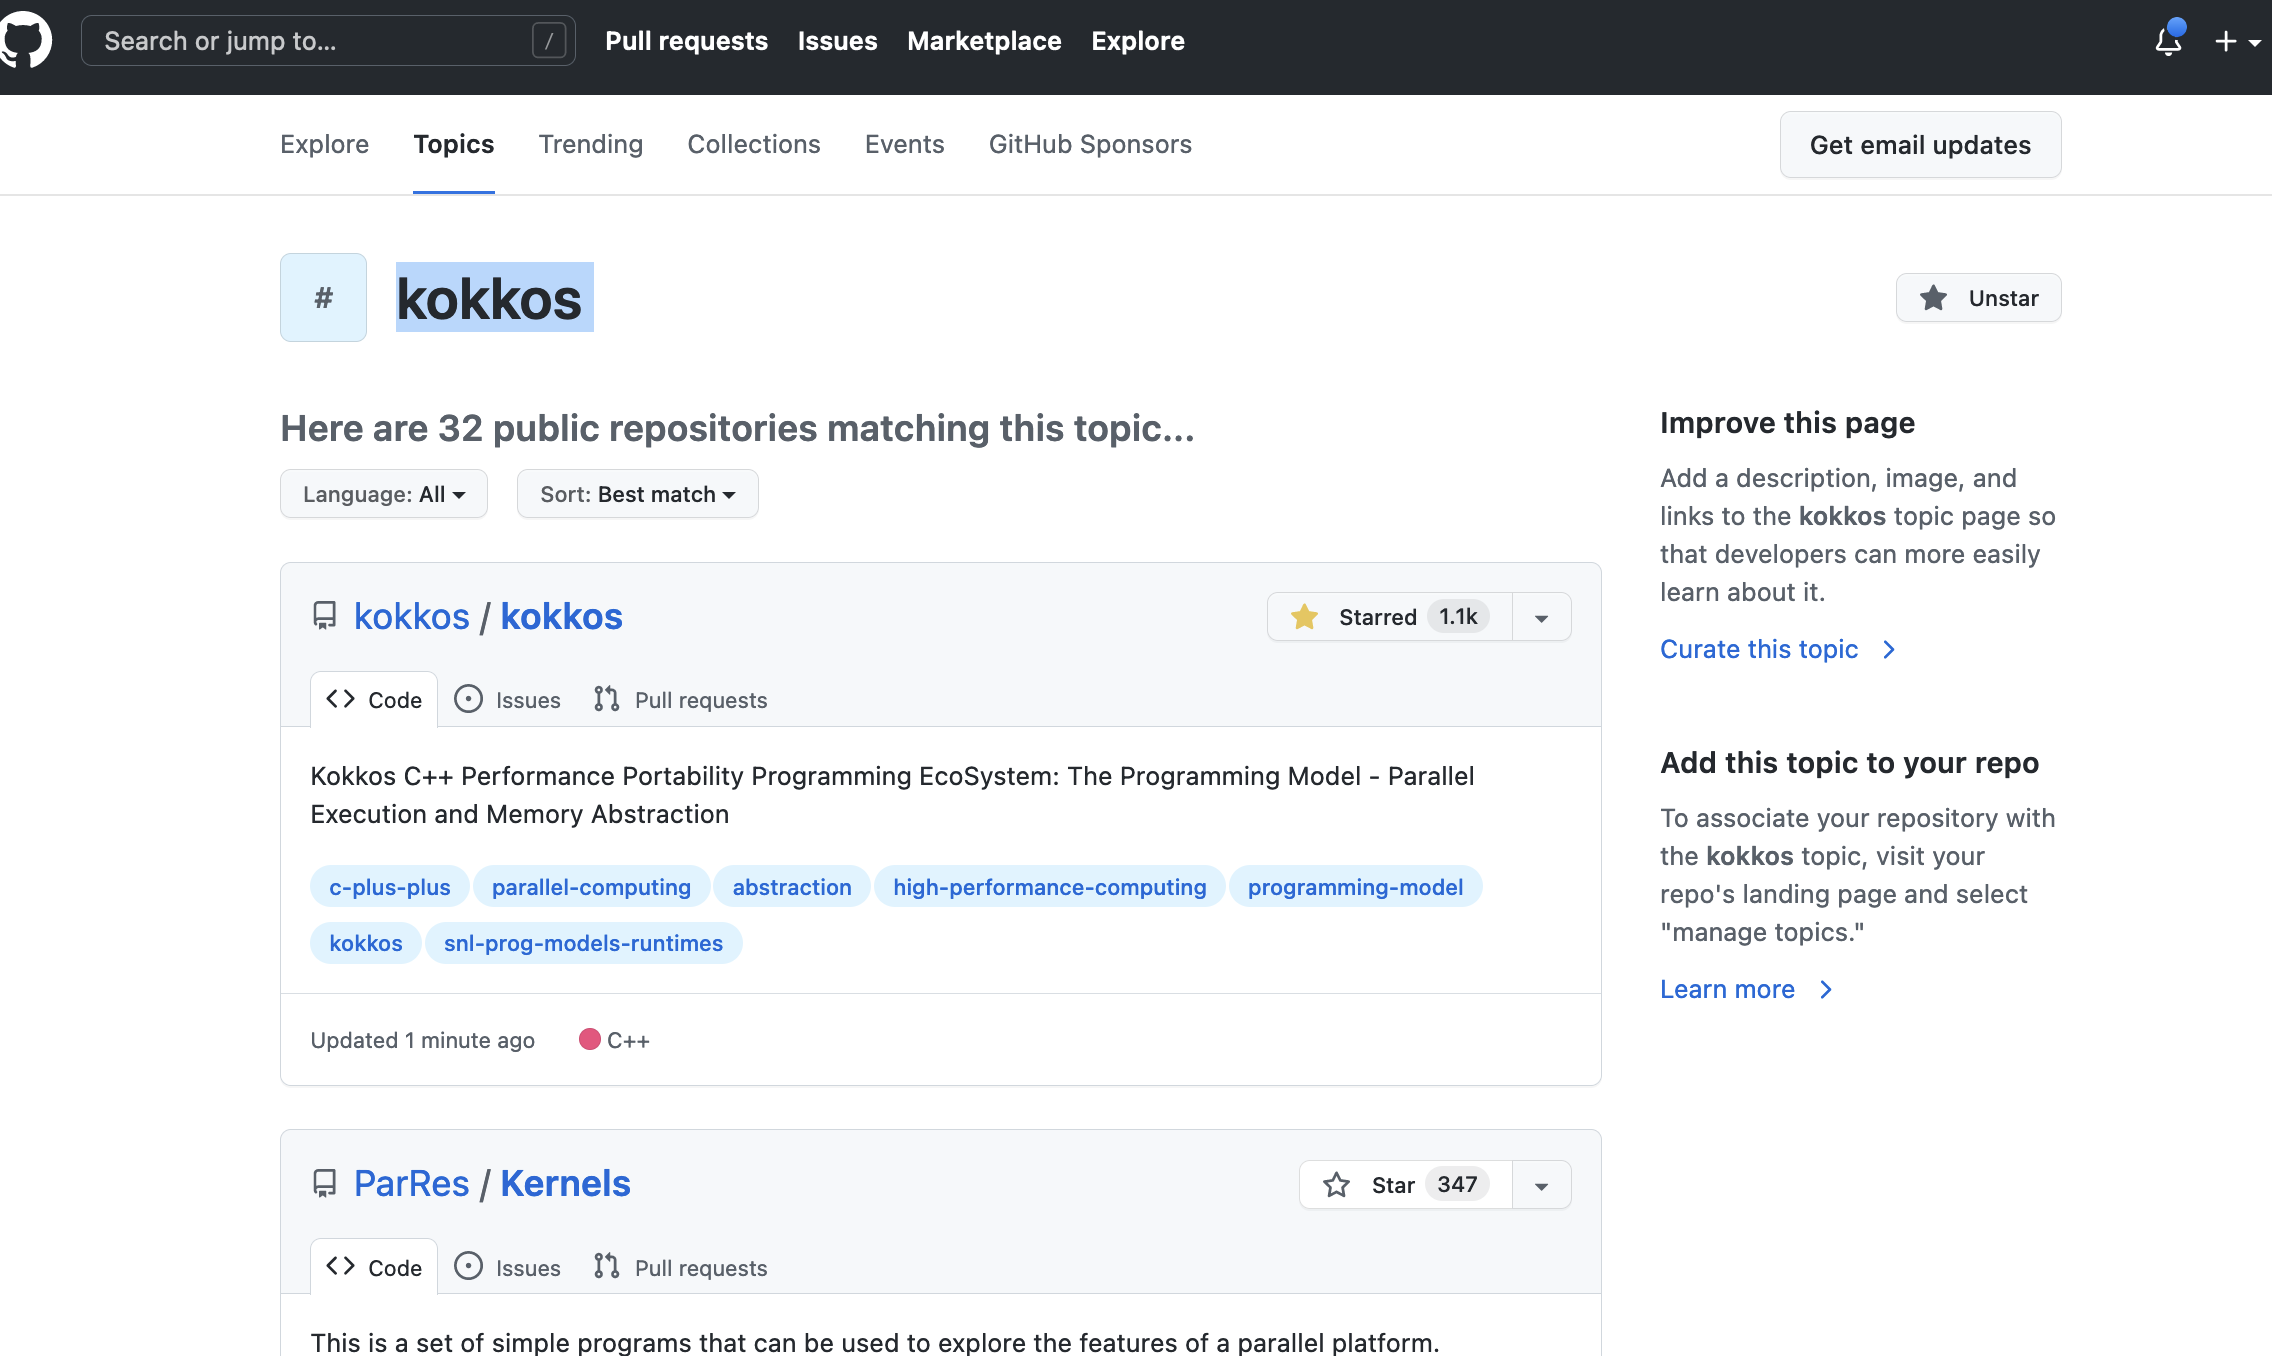
\includegraphics[width=0.9\textwidth]{3_7/kokkos-topic.png}
\end{frame}

\begin{frame}[fragile]{Kokkos user group meeting}
\begin{itemize}
\item We are considering organizing a multi-day in-person user group meeting 
\item Likely in Albuquerque
\item August/September time frame
\item Tentative content
   \begin{itemize}
   \item Updates from the Kokkos team (new features and planned work)
   \item User experiences: porting to AMD and Intel GPUs
   \item User experiences: performance portability studies
   \item Best practices (also user-provided)
   \item Students and Postdocs showcase
   \item Feedback and discussion session
   \end{itemize}
\end{itemize}
\vspace{10pt}
Lookout for survey to gauge interest
\end{frame}


%==========================================================================

\begin{frame}[fragile]{C++ Standard Change}
\textbf{Kokkos 4.0 requires C++17!}

\begin{itemize}
  \item {Supporting C++17, C++20 and C++23}
  \item {Allows us to keep the testing amount manageable}
  \item {Will enable new interfaces and streamlined implementation}
  \begin{itemize}
    \item {Use of CTAD reduces the need to spell template arguments out}
    \item {Fold expressions help with internal implementation, and improve compile times}
    \item {\texttt{constexpr if} reduces use of clunky SFINAE patterns}
  \end{itemize}
\end{itemize}
\end{frame}


\begin{frame}[fragile]{Toolchains minimum requirements change}
\textbf{New Compiler Minimums}

\vspace{10pt}
\small
\begin{tabular}{ll}
\textbf{Compiler} & \textbf{Version} \\
\hline
GCC & 8.2 \\
Clang & 8.0 \\
Clang as CUDA compiler & 10.0 \\
Intel & 19.0.5 \\
CUDA-NVCC & 11.0 \\
CUDA with Clang as CUDA compiler & 10.0.1 \\
ROCM & 5.2.0 \\
IntelLLVM (CPU) & 2021.1.1 \\
IntelLLVM (SYCL) & 2022.2.0 \\
NVC++ & 22.3 \\
MSVC & 19.29 \\
IBM XL & Not Supported \\
Classic PGI & Not Supported \\
\end{tabular}
\end{frame}

\begin{frame}[fragile]{A word on NVHPC}
\begin{itemize}
  \item NVIDIA is working on making NVC++ a single-pass CUDA compiler
  \item Kokkos 4 recognizes NVC++ as a CUDA compiler
  \item While tested, this is still experimental and several compiler bugs have been reported
  \item To use NVC++ as the host compiler with NVCC like before, you must use \texttt{nvcc\_wrapper} and pass \texttt{-ccbin nvc++} as cxx and linker flags or set the environment variable \texttt{NVCC\_WRAPPER\_DEFAULT\_COMPILER}
  \item Note as before, NVC++ does not use the GCC in your environment. You must create a configure file with \texttt{makelocalrc} pointing to a GCC supporting C++17
\end{itemize}
\end{frame}



%==========================================================================

\begin{frame}[fragile]

  {\Huge Backend Updates}

  \vspace{10pt}

  \textbf{Content:}
  \begin{itemize}
    \item Backend Updates Cuda
    \item Backend Updates HIP
    \item Backend Updates SYCL and OpenACC
  \end{itemize}

\end{frame}

%==========================================================================

\begin{frame}[fragile]{Backend Updates I}
\texttt{CUDA}
\begin{itemize}
    \item Fixed potential data race in \texttt{parallel\_reduce}
    \item Use \texttt{cudaMallocAsync} by default
    \item Bugfix when specifying non-default device ID while launching threads after initialization
    \item Deprecate \texttt{Cuda(cudaStream\_t,bool)} constructor
\end{itemize}
\end{frame}
\begin{frame}[fragile]{Backend updates II}
\texttt{HIP}
\begin{itemize}
    \item New naming convention:\\ \texttt{Kokkos\_ARCH\_VEGA90A} $\rightarrow$ \texttt{Kokkos\_ARCH\_AMD\_GFX90A}
    \item Add initial support for gfx942
    \item Add support for ROCM 5.5 and 5.6
    \item Improve reduction performance
    \item Fix potential data race in \texttt{HIP} \texttt{parallel\_reduce}
    \item Deprecate \texttt{HIP(hipStream\_t,bool)} constructor
    \item Add support for \texttt{Kokkos::Graph}
    \item Fix concurrency calculation
\end{itemize}
\end{frame}
\begin{frame}[fragile]{Backend Updates III}
\texttt{SYCL}
\begin{itemize}
    \item Enforce external \texttt{sycl::queues} to be in-order
    \item Make in-order \texttt{sycl::queues} the default via macro
    \item Improve reduction performance
    \item Allow using the \texttt{SYCL} execution space on AMD GPUs
    \item Allow sorting via native \texttt{oneDPL} to support \texttt{View}s with \texttt{stride=1}
\end{itemize}
\vfill
\texttt{OpenACC}
\begin{itemize}
    \item Add support for \texttt{clacc} compiler
\end{itemize}
\end{frame}

%==========================================================================



%==========================================================================


% Makefile and CMake support for C++23
% Update minimum compiler versions. (covered in earlier section)

\begin{frame}[fragile]{Build System Updates}
\textbf{C++ Standards Support}
\begin{itemize}
  \item \texttt{CMAKE\_CXX\_STANDARD=23} is supported
  \begin{itemize}
    \item \texttt{KOKKOS\_CXX\_STANDARD} for the Makefile
  \end{itemize}
  \item In CMake Kokkos will default to C++17 if no standard is specified
\end{itemize}
\end{frame}

%==========================================================================

% Let CMake determine OpenMP flags.
% Only add -latomic in generated GNU makefiles when OpenMPTarget backend is enabled

\begin{frame}[fragile]{Build System Updates}
\textbf{OpenMP and OpenMPTarget}
\begin{itemize}
  \item OpenMP flags are now determined by CMake's FindOpenMP
  \item Makefile: \texttt{libatomic} only linked in OpenMPTarget builds
\end{itemize}
\end{frame}

%==========================================================================

% Do not add -cuda to the link line with NVHPC compiler when the CUDA backend is not actually enabled
% Kokkos_ENABLE_CUDA_LAMBDA now ON by default with NVCC
% Fix enabling of relocatable device code when using CUDA as CMake language
% Fix cmake configuration with CUDA 12

\begin{frame}[fragile]{Build System Updates}
\textbf{CUDA}
\begin{itemize}
  \item \texttt{Kokkos\_ENABLE\_CUDA\_LAMBDA} set to \texttt{ON} by default
  \item Fixes to RDC flags when using CMake CUDA language
  \item Fixed CUDA 12 when using \texttt{nvcc\_wrapper} with CMake
  \item Fixes to using NVHPC as a compiler when CUDA is not enabled
\end{itemize}
\end{frame}

%==========================================================================



%==========================================================================

\begin{frame}[fragile]

  {\Huge Team- and Thread-Level (Nested) Sorting}

  \vspace{10pt}

  \textbf{Content:}
  Sorting routines that use nested parallelism
  \begin{itemize}
    \item Callable from within a TeamPolicy kernel
    \item Sort a View using the calling team or thread
    \begin{itemize}
      \item View may be in global or scratch memory
    \end{itemize}
    \item \texttt{sort}, \texttt{sort\_by\_key} functions
    \item Allow custom comparators
    \item In-place, not stable
  \end{itemize}

  \vspace{10pt}

  More sorting capabilities to come in the next releases.

\end{frame}

%==========================================================================

\begin{frame}[fragile]{Nested Sorting}

New functions:

\vspace{10pt}

\begin{itemize}
  \item \texttt{\#include "Kokkos\_NestedSort.hpp"}
  \item In namespace \texttt{Kokkos::Experimental}:
  \begin{itemize}
    \item \texttt{sort\_team(teamMem, view[, compare])}
    \item \texttt{sort\_by\_key\_team(teamMem, keys, values[, compare])}
    \item \texttt{sort\_thread(teamMem, view[, compare])}
    \item \texttt{sort\_by\_key\_thread(teamMem, keys, values[, compare])}
  \end{itemize}
\end{itemize}

\vspace{10pt}

\end{frame}

%==========================================================================

\begin{frame}[fragile]{Nested Sorting}

Arguments to new functions:

\vspace{10pt}

\begin{itemize}
  \item \texttt{teamMem}: the \texttt{TeamPolicy::member\_type} passed to your kernel
  \item \texttt{sort} functions take a single view
  \begin{itemize}
    \item \texttt{view}: a \texttt{View} to sort
  \end{itemize}
  \item \texttt{sort\_by\_key} functions sort key/value pairs according to key:
  \begin{itemize}
    \item \texttt{keys}: a \texttt{View} of keys to sort
    \item \texttt{values}: a \texttt{View} to permute along with the keys
  \end{itemize}
  \item \texttt{compare} (optional): a comparator object/predicate
  \begin{itemize}
    \item If not provided, sort ascending (\texttt{operator<})
    \item Otherwise: \texttt{compare(a, b)} returns true iff. \texttt{a} precedes \texttt{b}
    \begin{itemize}
      \item Defined as: \texttt{bool operator()(a, b) const}
    \end{itemize}
  \end{itemize}
\end{itemize}

\vspace{10pt}

\end{frame}



%==========================================================================

\begin{frame}[fragile]

  {\Huge Team-Level MDRange Policies}

  \vspace{10pt}

  \textbf{Content:}
  Provide multidimensional support for nested parallelism

\end{frame}

%==========================================================================

\begin{frame}[fragile]{TeamMDRangePolicies}

Additions to nested polcies:

\vspace{10pt}

\begin{itemize}
 \item MD versions of nested team execution policies
 \begin{itemize}
  \item Supports multi dimension in nested parallel pattern
 \end{itemize}
\end{itemize}

\vspace{10pt}

\begin{itemize}
 \item TeamThreadRange
 \item \textbf{TeamThreadMDRange}
 \item TeamVectorRange
 \item \textbf{TeamVectorMDRange}
 \item ThreadVectorRange
 \item \textbf{ThreadVectorMDRange}
\end{itemize}

\end{frame}

%==========================================================================

\begin{frame}[fragile]{\texttt{TeamMDRangePolicies API}}

API for TeamThreadMDRange, TeamVectorMDRange and ThreadVectorMDRange

\vspace{10pt}

\begin{code}[keywords={TeamVectorMDRange}]
 parallel_for(
   TeamVectorMDRange<Rank<2>, TeamHandle>(team_handle, N, M),
   [=](int i, int j) { /* ... */ }
 );
\end{code}

\vspace{10pt}

\begin{itemize}
  \item Takes in \texttt{Rank<N,OuterDir,InnerDir>} that describes its iteration pattern
  \item Same behavior as regular \texttt{MDRangePolicy}
  \begin{itemize}
    \item \texttt{N} is number of dimensions (required to be [2, 8])
    \item \texttt{Iterate} is an \texttt{enum \{ Default, Left, Right \}}
    \item \texttt{Iterate} is used to choose iterating left-most dimension or right-most dimension
    \item Only \texttt{OuterDir} is used for \texttt{TeamMDRange}
  \end{itemize}
\end{itemize}

%\begin{code}
%template <unsigned N, Iterate OuterDir = Iterate::Default,
%          Iterate InnerDir = Iterate::Default>
%struct Rank { /* ... */ };
%\end{code}

\end{frame}

%==========================================================================

\begin{frame}[fragile]{TeamThreadMDRange Example}

\begin{code}[keywords={TeamThreadMDRange}]
using TeamHandle = TeamPolicy<>::member_type;

parallel_for(TeamPolicy<>(N,AUTO),
             KOKKOS_LAMBDA (TeamHandle const& team) {
  int leagueRank = team.league_rank();
  auto teamThreadMDRange = TeamThreadMDRange<Rank<4>,
                           TeamHandle>(team, n0, n1, n2, n3);
  parallel_for(teamThreadMDRange,
    [=](int i0, int i1, int i2, int i3) {
      /* ... */
  });
}); 
\end{code}

\end{frame}

%==========================================================================

\begin{frame}[fragile]{ThreadVectorMDRange Example}

\begin{code}[keywords={ThreadVectorMDRange}]
using TeamHandle = TeamPolicy<>::member_type;

parallel_for(TeamPolicy<>(N, AUTO),
             KOKKOS_LAMBDA(TeamHandle const& team) { 
  int leagueRank = team.league_rank(); 
  auto teamThreadRange = TeamThreadRange(team, n0);
  auto threadVectorMDRange = ThreadVectorMDRange<Rank<3>,
                             TeamHandle>(team, n1, n2, n3);
  parallel_for(teamThreadRange, [=](int i0) {
    parallel_for(threadVectorMDRange,
      [=](int i1, int i2, int i3) {
        /* ... */
    });
  });
}); 
\end{code}

\end{frame}

%==========================================================================

\begin{frame}[fragile]{TeamVectorMDRange Example}

\begin{code}[keywords={TeamVectorMDRange}]
using TeamHandle = TeamPolicy<>::member_type;

parallel_for(TeamPolicy<>(N,AUTO),
             KOKKOS_LAMBDA(TeamHandle const& team) {
  int leagueRank = team.league_rank();
  auto teamVectorMDRange = TeamVectorMDRange<Rank<4>,
                           TeamHandle>(team, n0, n1, n2, n3);
  parallel_for(teamVectorMDRange,
    [=](int i0, int i1, int i2, int i3) {
      /* ... */
  });
}); 
\end{code}

\end{frame}

%==========================================================================

\begin{frame}[fragile]{TeamMDRangePolicies Notes}
\textit{Thread and Vector Parallelism:}

\begin{itemize}
  \item Based on iteration direction (\texttt{OuterDir})
  \item For now, at most 2 dimensions are parallelized
  \begin{itemize}
    \item Thread parallelism is applied to the slowest dimension
    \item Vector parallelism is applied to the fastest dimension
  \end{itemize}
\end{itemize}

\end{frame}

%==========================================================================


%==========================================================================

\begin{frame}[fragile]

  {\Huge SharedSpace}

  \vspace{10pt}

  \textbf{Content:}
  \begin{itemize}
    \item {\texttt{SharedSpace}}
    \item {\texttt{SharedPinnedHostSpace}}
  \end{itemize}

\end{frame}

%==========================================================================

\begin{frame}[fragile]{\texttt{SharedSpace} \& \texttt{SharedHostPinnedSpace}}

Aliases for \emph{\texttt{MemorySpaces}} that are accessible by every \emph{\texttt{ExecutionSpace}}.

\begin{description}
\item[\texttt{SharedSpace}] is memory that is moved and then accessed locally.
\item[\texttt{SharedHostPinnedSpace}] is memory that is pinned to the host and accessed via zero-copy access.
\end{description}

\begin{table}[htp]
%\caption{default}
\begin{center}
\begin{tabular}{| l | l | l |}
\hline
Backend & \texttt{SharedSpace} & \texttt{SharedHostPinnedSpace} \\
\hline \hline
CUDA & \texttt{CudaUVMSpace} & \texttt{CudaHostPinnedSpace} \\
\hline
HIP & \texttt{HIPManagedSpace} & \texttt{HIPHostPinnedSpace} \\
\hline
SYCL & \texttt{SYCLSharedUSMSpace} & \texttt{SYCLHostUSMSpace} \\
\hline
\emph{host} & \texttt{HostSpace} & \texttt{HostSpace} \\
\hline
\end{tabular}
\end{center}
\label{default}
\end{table}%



\end{frame}

%==========================================================================


\begin{frame}[fragile]{Miscellaneous}
\begin{itemize}
  \item Add \texttt{Kokkos::Profiling::ScopedRegion}
    \begin{code}	
     double myfunction()
     {
      Kokkos::Profiling::ScopedRegion region("foo");
      if (..)
        return bar;
      else
        return eval();
     }
    \end{code}
  \item Add support for \texttt{View::rank[\_dynamic]()}
  \item Detect incompatible relocatable device code mode to prevent ODR violations
  \item Add (experimental) support for 32-bit Darwin and PPC
  \item Add missing half and bhalf specialization of the infinity numeric trait
\end{itemize}
\end{frame}

\begin{frame}[fragile]{Miscellaneous}
\begin{itemize}
  \item Add \texttt{is\_dual\_view} trait and align template parameters with regular view
  \item Allow templated functors in \texttt{parallel\_for},
  \texttt{parallel\_reduce}, and \texttt{parallel\_scan}
  \item Define \texttt{KOKKOS\_COMPILER\_INTEL\_LLVM} and only define at most one
  \texttt{KOKKOS\_COMPILER*} macro
\end{itemize}
\end{frame}

%==========================================================================

%\begin{frame}[fragile]
%
%  {\Huge Drop volatile}
%
%  \vspace{10pt}
%
%  \textbf{Content:}
%  \begin{itemize}
%    \item {Drop \texttt{volatile} support from Atomic Views}
%  \end{itemize}
%
%\end{frame}

%==========================================================================
\begin{frame}[fragile]{Drop \texttt{volatile}}

\textbf{Drop \texttt{volatile} support from Atomic Views}

\vspace{20pt}

Historically, CUDA used \texttt{volatile} because it had a non-standard memory model.

This lead to problems when using custom types with Atomic Views.

\end{frame}

%==========================================================================

\begin{frame}[fragile]{Drop \texttt{volatile}}

\begin{code}

struct Custom {};
// ...
View<Custom[1], MemoryTraits<Atomic>> v(&a);
v[0] = a;

\end{code}

\begin{verbatim}
core/src/impl/Kokkos_Atomic_View.hpp:70: error:
passing ‘volatile AtomicDataElement<...>::value_type’ 
{aka ‘volatile Custom’} as ‘this’ argument discards
qualifiers [-fpermissive]
   70 |     *ptr = val;
      |     ~~~~~^~~~~
TestCustom.hpp: note: in call to
‘constexpr Custom& Custom::operator=(const Custom&)’
   |     struct Custom {};
   |            ^~~~~~
\end{verbatim}

\end{frame}

%==========================================================================

\begin{frame}[fragile]{Drop \texttt{volatile}}

Previously, one would have to add \texttt{volatile} declarations to their custom types:

\begin{code}
struct Custom {
    Custom& operator=(const Custom&) = default;
    void operator=(const Custom& src) volatile { /* ... */ }
    
    // As well as other volatile qualified member functions
};
\end{code}


However, internally Kokkos no longer uses the \texttt{volatile} overloads, and CUDA
no longer requires combining \texttt{volatile} with \texttt{atomic}.

\end{frame}

%==========================================================================

\begin{frame}[fragile]{Drop \texttt{volatile}}

Kokkos changes to internal \texttt{Impl::AtomicDataElement}:

\begin{itemize}
\item {Dropped \texttt{volatile} overloads}
\item {\texttt{operator=}  uses
\texttt{atomic\_store(..., memory\_order\_relaxed)}}
\item {\texttt{operator value\_type()} uses 
\texttt{atomic\_load(..., memory\_order\_relaxed)}}
\end{itemize}

Users
\begin{itemize}
\item {Drop the (now unused) \texttt{volatile} overloads at your convenience}
\end{itemize}

\end{frame}


 % merged into miscellaneous

%==========================================================================

\begin{frame}[fragile]

  {\Huge Deprecations}
  
    \vspace{10pt}

\end{frame}

\begin{frame}[fragile]{Deprecations}
\begin{itemize}
\item Deprecated allocation step inside \texttt{deep\_copy(UnorderedMap,UnorderedMap)}
  \begin{itemize}
    \item[] Maps now must have the same capacity to \texttt{deep\_copy}
  \end{itemize}
\item Deprecated implicit conversions of integers to \texttt{ChunkSize}
\begin{itemize}
  \item[] Behavior only introduced in 4.3
\end{itemize}
\item Deprecated implicit conversions to all execution spaces
\end{itemize}

\end{frame}

%==========================================================================

\begin{frame}[fragile]{Deprecate \texttt{Array<...,Proxy>} Argument}
\begin {itemize}
\item Deprecated trailing \texttt{Proxy} template argument in \texttt{Kokkos::Array}
\begin{code}
// DEPRECATED
// template <typename T = void,
//           size_t N = KOKKOS_INVALID_INDEX,
//           typename Proxy = void>
template <typename T, size_t N>
struct Array { /* ... */ };
\end{code}
  \begin{itemize}
    \item Deprecates \textit{non-owning, dynamically sized} \texttt{contiguous/strided} functionality
    \item More in line with (always) \textit{owning} \& \textit{statically sized} \texttt{std::array}
  \end{itemize}
\end{itemize}
\end{frame}

%==========================================================================

\begin{frame}[fragile]{Deprecate \texttt{is\_layouttiled}}
\begin {itemize}
\item Removed \texttt{Kokkos::Experimental::LayoutTiled} class template
  \begin{itemize}
  \item Never useable
  \end{itemize}
\item Deprecated \texttt{is\_layouttiled} trait
  \begin{itemize}
  \item Not useful, but no rush to remove it
  \end{itemize}
\item Deprecated \texttt{Kokkos::layout\_iterate\_type\_selector}
  \begin{itemize}
  \item Not useful outside of Kokkos implementation
  \end{itemize}
\end{itemize}
\end{frame}

%==========================================================================
\begin{frame}[fragile]{Deprecate \texttt{pair<T,void>}}
\begin {itemize}
\item Deprecated specialization of \texttt{Kokkos::pair} for a single element
\begin{code}
// DEPRECATED
// template <typename T>
// struct pair<T, void> { /* ... */ };
\end{code}
  \begin{itemize}
  \item Never supported in \texttt{std::pair}
  \item Never documented
  \item Never tested
  \item No known usage
  \end{itemize}
\end{itemize}
\end{frame}

%==========================================================================



\end{document}


